% Reusable figures for the project.
% Insert a figure in a document by calling its named command.

\definecolor{auctionRoomOne}{RGB}{225,236,247}
\definecolor{auctionRoomTwo}{RGB}{232,243,228}
\definecolor{auctionOutside}{RGB}{245,241,232}
\definecolor{auctionSunny}{RGB}{45,76,105}
\definecolor{auctionRainy}{RGB}{156,78,53}
\definecolor{auctionEquilibrium}{RGB}{224,183,74}

% Common axes for the two-good price diagrams.
\newcommand{\AuctionPriceAxes}{%
    \draw[-stealth,thick] (0,0) -- (64,0) node[right] {$p_1$};
    \draw[-stealth,thick] (0,0) -- (0,64) node[above] {$p_2$};
    \foreach \x in {10,20,...,60}
        \draw (\x,0.8) -- (\x,-0.8) node[below] {\scriptsize \x};
    \foreach \y in {10,20,...,60}
        \draw (0.8,\y) -- (-0.8,\y) node[left] {\scriptsize \y};
}

\newcommand{\SunnyDemandFigure}{%
    \begin{figure}[ht]
        \centering
        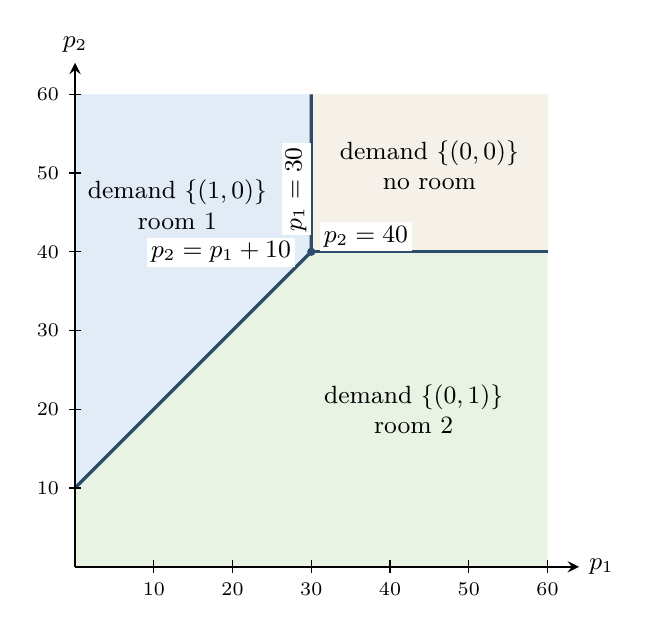
\begin{tikzpicture}[x=0.1cm,y=0.1cm,
            every node/.style={font=\small}]
            % Demand regions in the nonnegative price orthant.
            \fill[auctionRoomOne]
                (0,10) -- (0,60) -- (30,60) -- (30,40) -- cycle;
            \fill[auctionOutside]
                (30,40) -- (30,60) -- (60,60) -- (60,40) -- cycle;
            \fill[auctionRoomTwo]
                (0,0) -- (60,0) -- (60,40) -- (30,40) -- (0,10) -- cycle;

            % Locus of indifference prices.
            \draw[auctionSunny,very thick]
                (0,10) -- (30,40) -- (30,60);
            \draw[auctionSunny,very thick] (30,40) -- (60,40);
            \fill[auctionSunny] (30,40) circle[radius=1.5pt];

            \AuctionPriceAxes

            % Region and boundary labels.
            \node[align=center] at (13,46) {demand $\{(1,0)\}$\\room 1};
            \node[align=center] at (43,20) {demand $\{(0,1)\}$\\room 2};
            \node[align=center] at (45,51) {demand $\{(0,0)\}$\\no room};
            \node[anchor=south east,fill=white,inner sep=1.5pt]
                at (28,38) {$p_2=p_1+10$};
            \node[anchor=south west,fill=white,inner sep=1.5pt]
                at (31,40) {$p_2=40$};
            \node[anchor=south west,fill=white,inner sep=1.5pt,rotate=90]
                at (30,42) {$p_1=30$};
        \end{tikzpicture}
        \caption{Sunny's demand as a function of the price vector
        $p=(p_1,p_2)$. On the dark boundary, Sunny is indifferent between
        the adjacent labeled bundles.}
        \label{fig:sunny-demand}
    \end{figure}%
}

\newcommand{\RainyDemandFigure}{%
    \begin{figure}[ht]
        \centering
        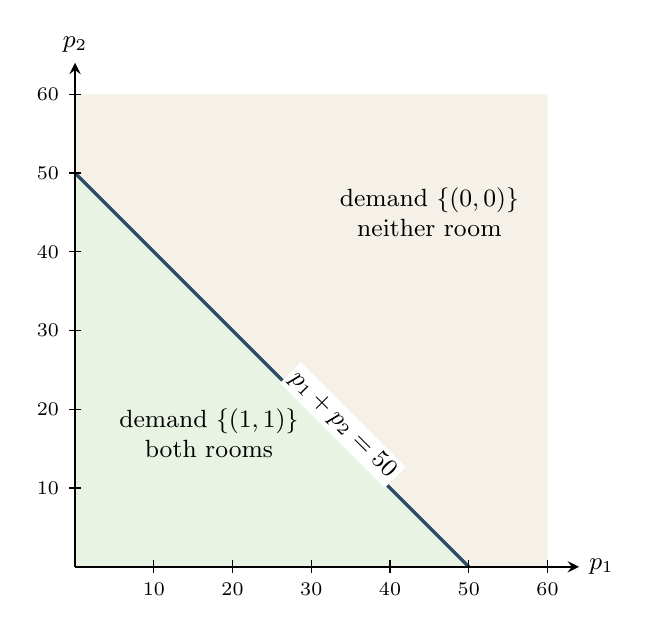
\begin{tikzpicture}[x=0.1cm,y=0.1cm,
            every node/.style={font=\small}]
            % Demand regions in the nonnegative price orthant.
            \fill[auctionRoomTwo] (0,0) -- (50,0) -- (0,50) -- cycle;
            \fill[auctionOutside]
                (0,50) -- (0,60) -- (60,60) -- (60,0) -- (50,0) -- cycle;

            % Locus of indifference prices.
            \draw[auctionSunny,very thick] (0,50) -- (50,0);

            \AuctionPriceAxes

            % Region and boundary labels.
            \node[align=center] at (17,17) {demand $\{(1,1)\}$\\both rooms};
            \node[align=center] at (45,45) {demand $\{(0,0)\}$\\neither room};
            \node[fill=white,inner sep=1.5pt,rotate=-45] at (34,18)
                {$p_1+p_2=50$};
        \end{tikzpicture}
        \caption{Rainy's demand as a function of the price vector
        $p=(p_1,p_2)$. Along the dark line, Rainy is indifferent between
        buying both rooms and buying neither.}
        \label{fig:rainy-demand}
    \end{figure}%
}

\newcommand{\CombinedDemandFigure}{%
    \begin{figure}[ht]
        \centering
        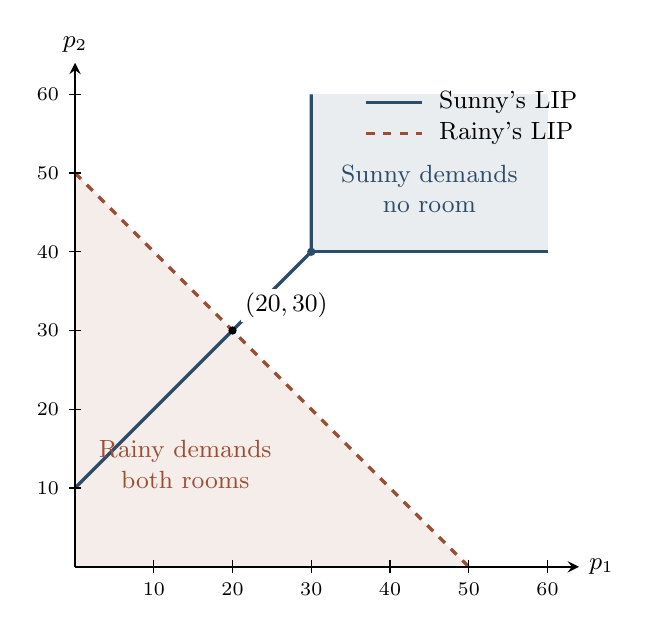
\begin{tikzpicture}[x=0.1cm,y=0.1cm,
            every node/.style={font=\small}]
            % Regions needed for the only market-clearing allocation:
            % Sunny takes no room and Rainy takes both rooms.
            \fill[auctionSunny,opacity=0.10]
                (30,40) -- (30,60) -- (60,60) -- (60,40) -- cycle;
            \fill[auctionRainy,opacity=0.10]
                (0,0) -- (50,0) -- (0,50) -- cycle;

            % Sunny's and Rainy's loci of indifference prices.
            \draw[auctionSunny,very thick]
                (0,10) -- (30,40) -- (30,60);
            \draw[auctionSunny,very thick] (30,40) -- (60,40);
            \fill[auctionSunny] (30,40) circle[radius=1.5pt];
            \draw[auctionRainy,very thick,dashed] (0,50) -- (50,0);

            % Unique intersection of the two demand complexes.
            \fill[black] (20,30) circle[radius=1.5pt];
            \node[anchor=south west,fill=white,inner sep=1.5pt]
                at (21,31) {$(20,30)$};

            \AuctionPriceAxes

            % Regions relevant to market clearing.
            \node[auctionSunny,align=center] at (45,48)
                {Sunny demands\\no room};
            \node[auctionRainy,align=center] at (14,13)
                {Rainy demands\\both rooms};

            % Line style also distinguishes the agents in grayscale.
            \draw[auctionSunny,very thick] (37,59) -- (44,59);
            \node[anchor=west] at (45,59) {Sunny's LIP};
            \draw[auctionRainy,very thick,dashed] (37,55) -- (44,55);
            \node[anchor=west] at (45,55) {Rainy's LIP};
        \end{tikzpicture}
        \caption{The superposed demand complexes. The lightly shaded regions
        show the price vectors at which Sunny demands no room and Rainy
        demands both rooms, respectively. Their disjointness rules out the
        only allocation that could clear the market.}
        \label{fig:combined-demand}
    \end{figure}%
}

\newcommand{\UpdatedCombinedDemandFigure}{%
    \begin{figure}[ht]
        \centering
        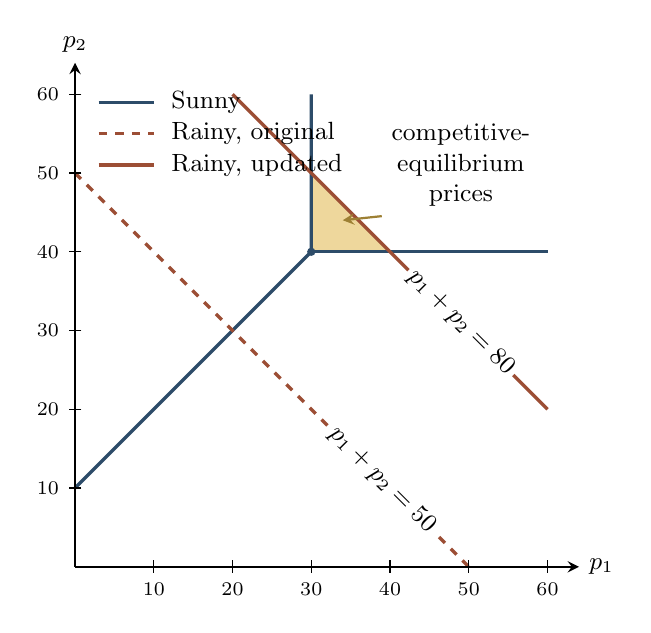
\begin{tikzpicture}[x=0.1cm,y=0.1cm,
            every node/.style={font=\small}]
            % Competitive-equilibrium prices satisfy
            % p_1 >= 30, p_2 >= 40, and p_1 + p_2 <= 80.
            \fill[auctionEquilibrium,opacity=0.55]
                (30,40) -- (30,50) -- (40,40) -- cycle;
            \draw[auctionEquilibrium!70!black,thick]
                (30,40) -- (30,50) -- (40,40) -- cycle;

            % Sunny's locus of indifference prices.
            \draw[auctionSunny,very thick]
                (0,10) -- (30,40) -- (30,60);
            \draw[auctionSunny,very thick] (30,40) -- (60,40);
            \fill[auctionSunny] (30,40) circle[radius=1.5pt];

            % Rainy's original and updated loci of indifference prices.
            \draw[auctionRainy,very thick,dashed] (0,50) -- (50,0);
            \draw[auctionRainy,very thick] (20,60) -- (60,20);

            \AuctionPriceAxes

            % Compact legend.
            \draw[auctionSunny,very thick] (3,59) -- (10,59);
            \node[anchor=west] at (11,59) {Sunny};
            \draw[auctionRainy,very thick,dashed] (3,55) -- (10,55);
            \node[anchor=west] at (11,55) {Rainy, original};
            \draw[auctionRainy,very thick] (3,51) -- (10,51);
            \node[anchor=west] at (11,51) {Rainy, updated};

            \node[fill=white,inner sep=1.5pt,rotate=-45] at (39,11)
                {$p_1+p_2=50$};
            \node[fill=white,inner sep=1.5pt,rotate=-45] at (49,31)
                {$p_1+p_2=80$};
            \node[align=center] (equilibriumLabel) at (49,51)
                {competitive-\\equilibrium\\prices};
            \draw[-stealth,auctionEquilibrium!70!black,thick]
                (equilibriumLabel.south west) -- (34,44);
        \end{tikzpicture}
        \caption{The demand complexes after Rainy's value for the pair rises
        from $50$ to $80$. Her original indifference line is dashed, while
        the solid line is her updated locus of indifference prices. The
        shaded triangle is the set of competitive-equilibrium prices.}
        \label{fig:updated-combined-demand}
    \end{figure}%
}
